\section{实验准备}

\subsection{代码包介绍}

\subsubsection{目录介绍}


\begin{table}[H]
    \begin{tabularx}{1\textwidth}{ l X } % | 表示垂直边框
        \hline % 水平边框
        \textbf{目录名} & \textbf{介绍}  \\
        \hline
        dqn&dqn 算法子目录\\
        target\_dqn&target\_dqn 算法子目录\\
        diy&Do it yourself 用户自定义算法的子目录\\
        conf&配置文件\\
        train\_test.py&代码正确性测试脚本\\
        \hline
    \end{tabularx}

    \centering
    \caption{代码目录}
    \label{directory}
\end{table}

其中 dqn,target\_dqn 是重返秘境场景的 2 个核心算法,diy为用户自定义的算法。各个算法的子目录结构如下:

\begin{table}[H]
    \begin{tabularx}{1\textwidth}{ l X } % | 表示垂直边框
        \hline % 水平边框
        \textbf{目录名/文件名} & \textbf{介绍}  \\
        \hline
        algorithm/&算法相关,主要是 agent 的实现,包含训练和预测,详情见算法开发\\
        feature/&特征相关,主要包含用户自定义的数据结构和数据处理方法,以及特征和奖励的计算,详情见实现特征处理和样本处理\\
        model/&模型相关,主要是模型的实现,是一个Model类\\
        config.py&该算法下的配置,用户可以任意增加配置或修改配置,注意:SAMPLE\_DIM是开悟框架使用配置,不允许删除\\
        train\_workflow.py&强化学习的训练流程,详情见强化学习训练流程开发        \\
        \hline
    \end{tabularx}

    \centering
    \caption{自定义算法}
    \label{directory:alg}
\end{table}


\subsection{开发流程}

概括来说,我们的开发任务是:开发智能体和智能体的训练流程,这个智能体包含一个可被训练的模型,智能体可以对环境给出的观测进行决策,这个决策作用于环境产生新的观测,此过程通过训练流程控制,不断循环。训练流程还要收集循环过程中产生的每一帧数据,将他们组合成样本数据,智能体可以根据这些样本作为算法的输入,通过算法更新模型。由于重返秘境采用分布式训练,会启动多个容器,样本需要通过网络通信发送到训练容器(learner)中进行训练,所以需要对样本进行编码方便网络发送,另外智能体需要将learner容器上的模型同步回来。以上任务可以描述为 \Cref{dev-process}:

\begin{figure}[H]
    \centering
    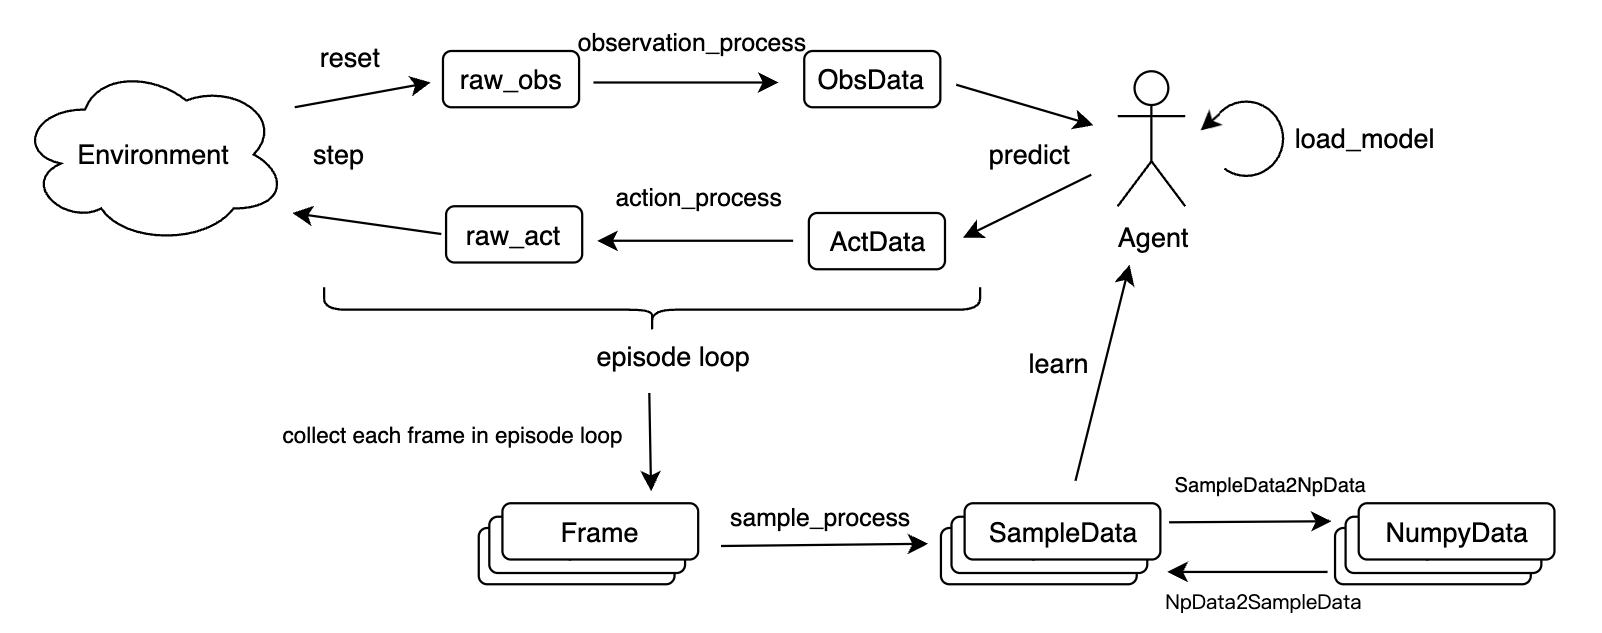
\includegraphics[width=1\linewidth]{pic/dev-process.png}
    \caption{\zihao{-5} 开发流程}
    \label{dev-process}
\end{figure}

开发流程如下:

\begin{enumerate}
\item 定义数据结构:一般情况下,环境产生的原始观测数据不能直接作为智能体的输入,并且不同的用户开发的智能体一般是不一样的,显然不同的智能体的决策、学习方法的输入输出也是不一样的,所以开发的第一步,我们应该定义智能体输入输出的数据结构。包括特征(ObsData)、动作(ActData)、样本(SampleData),其中ObsData和ActData分别作为智能体predict方法的输入和输出,SampleData作为智能体learn方法的输入。
\item 实现特征处理和样本处理:不同的用户实现不同的智能体可能会定义不同的数据结构,但是,环境接口输入输出的数据结构是固定的,因此环境接口的输入输出数据和智能体接口的输入输出数据需要进行转换,所以还需要用户实现这些数据结构的转换方法,包括:observation\_process, action\_process, sample\_process。
\item 算法开发:用户需要实现一个 agent,agent中实现一个模型(一般是神经网络模型)。agent负责与环境交互,产生预测动作并训练模型。
\item 实现强化学习训练流程:在实现了 数据结构,数据处理函数,模型和 智能体 以及其他方法(如奖励处理函数)后,我们还需要实现一个强化学习的训练流程workflow,将所有组件组合起来完成强化学习训练,即智能体通过不断的与环境交互,获取样本数据,更新并迭代模型,直到模型收敛到我们想要的效果。
\item 训练参数配置:在分布式训练时,开悟平台会启动一个样本池,一个模型同步服务,这些组件的相关参数用户可以根据自己的设计进行配置
\end{enumerate}


\begin{figure}[H]
    \centering
    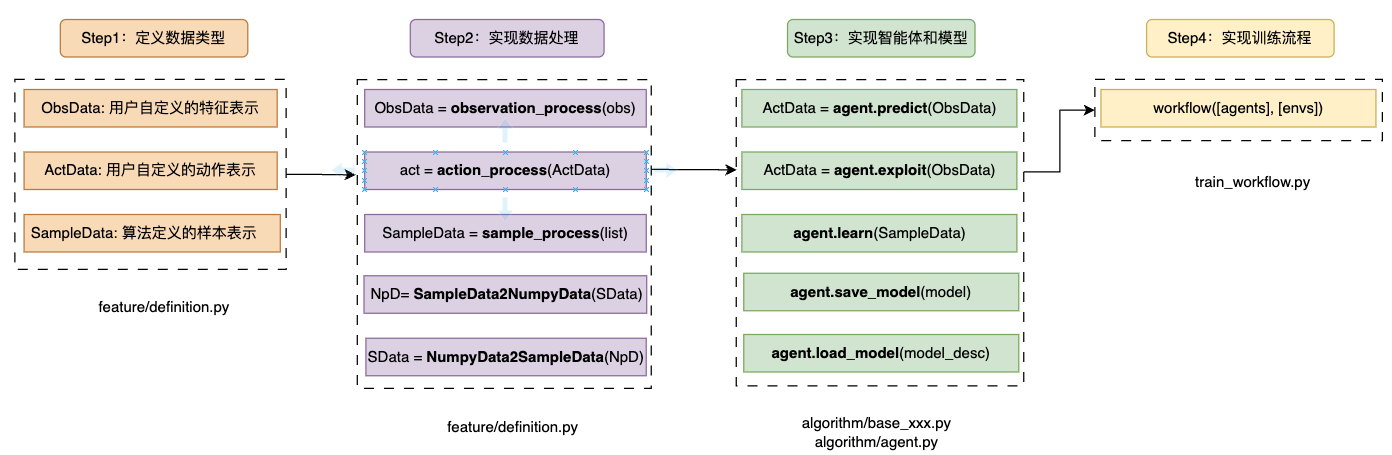
\includegraphics[width=1\linewidth]{pic/dev-process-1.png}
    \caption{\zihao{-5} 开发流程}
    \label{dev-process-1}
\end{figure}

分布式训练架构如 \Cref{train} 所示,

\begin{figure}[H]
    \centering
    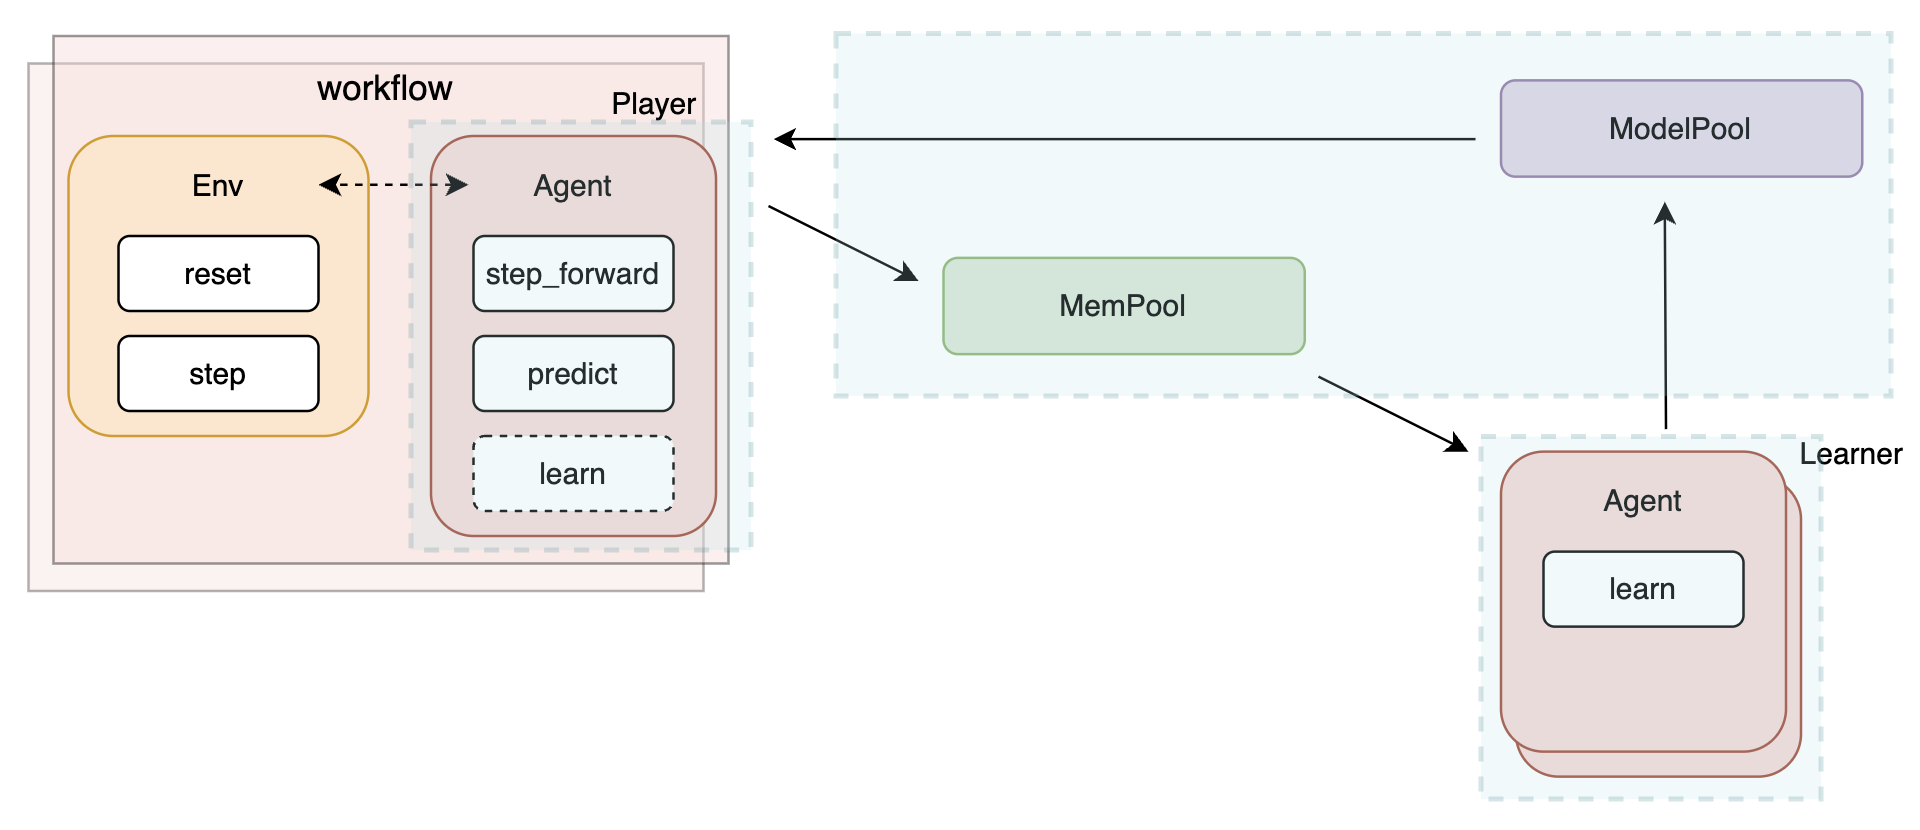
\includegraphics[width=1\linewidth]{pic/train.png}
    \caption{\zihao{-5} 分布式训练架构}
    \label{train}
\end{figure}

特别注意: 因为重返秘境会进行分布式训练,开悟平台会启动一个样本池(样本先进先出),用户的agent.learn(samples)调用将会把样本发送到样本池,训练容器会从样本池中采样样本samples将其传入agent.learn(samples)进行训练,此过程是自动的,用户无需开发额外代码.

\subsubsection{定义数据结构}

环境介绍里详细描述了环境返回的原始观测信息 obs,这里的 obs 已经做了一定的数据预处理工作,但是智能体是由用户设计和实现的,环境使用的obs, act等与智能体的输入输出是存在差异的,所以要先定义数据结构(类)再进行数据转换,包括:包括特征(ObsData)、动作(ActData)、样本(SampleData),这部分的代码,都需要实现在<算法名称>/feature/definition.py中。

我们以 DQN 算法为例,介绍解决环境配置为固定宝箱时的数据类型定义。

首先需要定义相关的数据结构(类)包含观测数据ObsData,动作数据ActData,和样本数据SampleData, 其中ObsData和ActData分别表示智能体预测的输入和输出,将会由agent.predict使用;SampleData为样本的数据类型,样本数据将会被agent.learn中的代码进行处理用于模型的训练。这些数据结构(类)包含哪些属性完全由用户自定义,属性名称属性数量没有限制。

create\_cls函数用于动态创建一个类,create\_cls的第一个参数为类型名称,剩余参数为类的属性,属性默认值为None。以下是代码示例:

\begin{lstlisting}[language=Python]
# The create_cls function is used to dynamically create a class. The first parameter of the function is the type name,
# and the remaining parameters are the attributes of the class, which should have a default value of None.
# create_cls函数用于动态创建一个类,函数第一个参数为类型名称,剩余参数为类的属性,属性默认值应设为None
ObsData = create_cls("ObsData",
    feature=None,
    legal_act=None)

ActData = create_cls("ActData",
    move_dir=None,
    use_talent=None)

SampleData = create_cls("SampleData",
    obs=None,
    _obs=None,
    obs_legal=None,
    _obs_legal=None,
    act=None,
    rew=None,
    ret=None,
    done=None) 
\end{lstlisting}

\subsubsection{实现特征处理和样本处理}

用户需要实现特征处理,动作处理,样本处理,和奖励设计函数,例如环境返回的数据属于原始观测数据,是无法直接作为智能体预测时的输入的,我们需要实现特征处理函数(observation\_process),将环境返回的原始观测数据转换成用户定义的ObsData。这部分的代码,都需要实现在<算法名称>/feature/definition.py中。

我们依然以 DQN算法为例,介绍解决环境配置为固定宝箱时的特征处理和样本处理。

需要实现特征处理和样本处理的函数有:observation\_process, action\_process, sample\_process。


\begin{table}[H]
    \begin{tabularx}{1\textwidth}{ X X X X } % | 表示垂直边框
        \hline % 水平边框
        \textbf{函数名} & \textbf{输入} & \textbf{输出} & \textbf{描述} \\
        \hline
        observation\_process&env.reset和env.step返回的原始观测数据raw\_obs&用户定义的ObsData类型的数据&将环境返回的原始观测数据转换成用户定义的ObsData类型数据\\
        action\_process&用户定义的ActData类型的数据&env.step能处理的动作数据&将智能体预测返回的ActData类的数据转换成env.step能处理的动作数据\\
        sample\_process&在环境中收集的每一帧信息组成的列表&SampleData类型的数据组成的列表&将环境数据帧的集合转换为样本的集合\\
        \hline
    \end{tabularx}

    \centering
    \caption{函数描述}
    \label{functions}
\end{table}

\subsubsection{奖励设计}

这里的奖励特指强化学习中的Reward,注意要与项目简介中的计分规则区别开。任务得分用于衡量玩家在任务中的表现,也作为衡量强化学习训练后的模型的优劣。代码包里提供了一些奖励的实现,可以参考这部分代码<算法名称>/feature/definition.py里的reward\_shaping函数修改各个奖励的权重。
不仅可以设置权重,还可以在<算法名称>/feature/definition.py里的reward\_shaping函数去实现自己的reward设计。

\subsubsection{算法开发}

重返秘境目前支持以下算法:DQN,Target-DQN,另外,我们还留了一个未实现的算法DIY,提供给用户进行自定义算法的实现,以上每个算法的开发流程都是一致的,所以这里以 DQN 的代码为例,讲解 DQN 是如何实现的:

首先,如果我们需要实现一个神经网络模型,我们需要在文件<算法名称>/model/model.py中实现一个Model类,即用pytorch实现一个神经网络模型。

然后,我们需要在文件<算法名称>/algorithm/agent.py中实现一个 Agent类。注意Agent类需要继承 kaiwu\_agent.agent.base\_agent 的 BaseAgent 类,Agent类的实现需要符合BaseAgent类的接口规范

注意:Agent类必须使用@attached装饰器,代码默认已实现,注意不要删除。


\begin{lstlisting}[language=Python]
    class BaseAgent:
    """
    Agent 的基类,所有的 Agent 都应该继承自这个类"""
    def __init__(self, agent_type="player", device=None, logger=None, monitor=None) -> None:
        raise NotImplementedError

    def learn(self, list_sample_data) -> dict:
        """
        用于学习的函数,接受一个 SampleData 的列表
        """
        raise NotImplementedError

    def predict(self, list_obs_data: list) -> list:
        """
        用于获取动作的函数,接受一个 ObsData 的列表, 返回一个动作列表
        """
        raise NotImplementedError

    def exploit(self, list_obs_data: list) -> list:
        """
        用于获取动作的函数,接受一个 ObsData 的列表, 返回一个动作列表
        """
        raise NotImplementedError

    def save_model(self, path, id='1'):
        raise NotImplementedError

    def load_model(self, path, id='1'):
        raise NotImplementedError
\end{lstlisting}

Agent类有三个核心的方法predict,exploit,和learn,其中predict和exploit方法负责进行预测,区别在于前者是智能体训练时调用的方法,一般是依策略的概率分布采样或引入随机概率,后者是智能体在评估时调用的方法,一般是选取策略中概率最高的动作或者策略认为最优的动作;learn方法中实现了核心算法,主要负责消费样本进行模型训练,其示例代码如下:

\begin{lstlisting}[language=Python]
"""
DQN/algorithm/agent.py
"""
@attached
class Agent(base_dqn.Agent):
    def __init__(self, agent_type="player", device="cpu", logger=None, monitor=None):
        # 进行若干初始化操作
        # ...

    @predict_wrapper
    def predict(self, list_obs_data):
        return self.__predict_detail(list_obs_data, exploit_flag=False)

    @exploit_wrapper
    def exploit(self, list_obs_data):
        return self.__predict_detail(list_obs_data, exploit_flag=True)

    @learn_wrapper
    def learn(self, list_sample_data):
        # 算法详细代码不在此处展示
\end{lstlisting}


\subsubsection{强化学习流程}

在实现了 数据结构,数据处理函数,模型和 智能体 以及其他方法(如奖励处理函数)后,我们还需要实现一个强化学习的训练流程workflow将所有组件结合起来完成强化学习训练,即智能体通过不断的与环境交互,获取样本数据,更新并迭代模型,直到模型收敛。

完成了上述组件之后,需要再实现一个强化学习的训练流程workflow,来让智能体 Agent 和环境 Environment 不断的交互从而产生。


\begin{figure}[H]
    \centering
    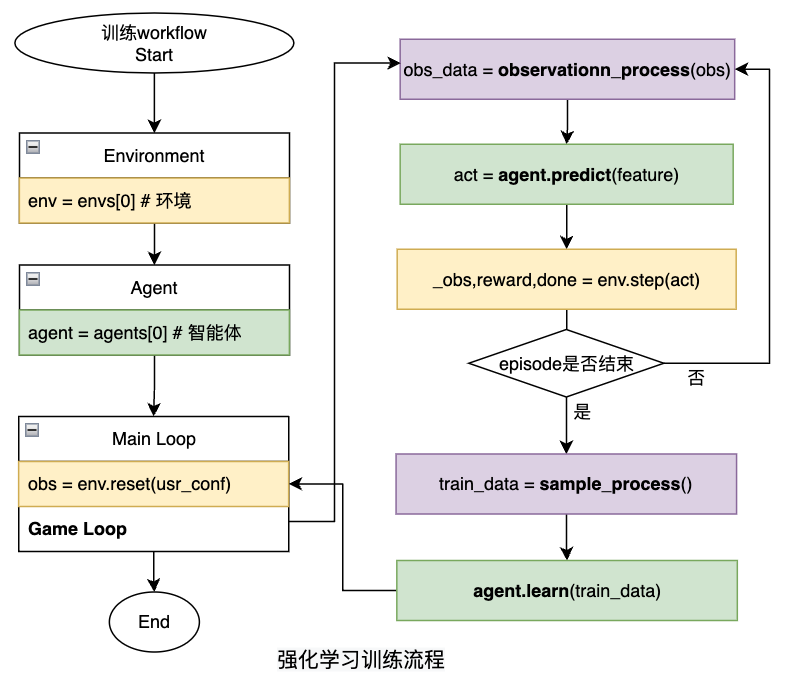
\includegraphics[width=0.8\linewidth]{pic/reinforcement.png}
    \caption{\zihao{-5} 强化学习流程}
    \label{reinforcement}
\end{figure}
